\documentclass{article}

\usepackage{iclr2026_conference,times}
\usepackage{fontspec}
\setmainfont[
  Path=fonts/,
  UprightFont=STIXGeneral.ttf,
  BoldFont=STIXGeneralBol.ttf,
  ItalicFont=STIXGeneralItalic.ttf,
  BoldItalicFont=STIXGeneralBolIta.ttf
]{STIXGeneral}
\setmonofont[
  Path=fonts/,
  UprightFont=DejaVuSansMono.ttf,
  BoldFont=DejaVuSansMono-Bold.ttf,
  ItalicFont=DejaVuSansMono-Oblique.ttf,
  BoldItalicFont=DejaVuSansMono-BoldOblique.ttf
]{DejaVuSansMono}
\usepackage{amsmath,amssymb,booktabs,graphicx,microtype,tabularx}
\usepackage{array}
\usepackage[hidelinks]{hyperref}

\newcolumntype{L}[1]{>{\raggedright\arraybackslash}p{#1}}
\newcolumntype{Y}{>{\raggedright\arraybackslash}X}

% Compact, readable float spacing; the official style and body font are unchanged.
\setlength{\parskip}{4pt plus 0.5pt minus 0.5pt}
\setlength{\textfloatsep}{6pt plus 1pt minus 1pt}
\setlength{\floatsep}{5pt plus 1pt minus 1pt}
\setlength{\intextsep}{6pt plus 1pt minus 1pt}
\setlength{\abovecaptionskip}{3pt}
\setlength{\belowcaptionskip}{0pt}
\setlength{\abovedisplayskip}{5pt plus 2pt minus 2pt}
\setlength{\belowdisplayskip}{5pt plus 2pt minus 2pt}
\emergencystretch=1em

\graphicspath{{figures/}}
\newcommand{\dllm}{diffusion language model}
\newcommand{\dLLM}{diffusion language model}
\newcommand{\armA}{AR-init}
\newcommand{\armB}{random-init}
\newcommand{\shachunks}[8]{\texttt{#1}\allowbreak\texttt{#2}\allowbreak\texttt{#3}\allowbreak\texttt{#4}\allowbreak\texttt{#5}\allowbreak\texttt{#6}\allowbreak\texttt{#7}\allowbreak\texttt{#8}}

\title{Reporting Degenerate Emissions in a 135M Diffusion Language Model:\\
A Reproducible Negative-Control Pilot}

\author{Anonymous authors}

\begin{document}

\maketitle

\begin{abstract}
We examine a negative control on one 135M-parameter masked diffusion language
model bed.  Under a matched short budget, autoregressive initialization has a
2.26-nat lower last-logged loss than one fixed random initialization, with the
same direction across four paired data-order seeds.  Because the random
initialization is a single fixed draw, these repeats do not measure
weight-draw variance.  In a single-prompt generation pilot, both arms are
visibly degenerate.  Teacher perplexity ranks them opposite to the paired loss
benchmark, whereas effective length, alphabetic yield, and emitted-token
concentration distinguish their emissions.  Neither comparison establishes a
quality ranking or metric capability because the pilot has no independent
quality anchor.  MAUVE is \emph{not recorded} under this configuration, so we
form no ratio and draw no MAUVE inference.  The resulting engineering
deliverable is a companion record that places emission length and degeneration
beside per-token scores; it is not a new scalar metric, training method, or
claim beyond this bed.
\end{abstract}

\section{Introduction}
\label{sec:introduction}

Masked diffusion language models generate by repeatedly denoising a canvas of
masked tokens rather than extending a causal prefix one token at a time
\citep{sahoo2024mdlm,nie2025llada}.  This design exposes intermediate
signals---entropy, maximum probability, mask state, and changes in the current
argmax---that can guide adaptive decoding \citep{li2025daedal}.  Generated-text
PPL, MAUVE, and trajectory summaries describe different projections of an
emission; none is an independent human-quality anchor in our experiment.
Wang et al.\ diagnose length, repetition, and punctuation as factors that can
distort PLM-based perplexity \citep{wang2022ppl}.  We therefore ask only whether
two known-degenerate outputs in one small dLLM pilot differ on analogous
emission fields that our initial report did not place beside each score.

This paper turns a small training bed into a controlled negative-control pilot
case study.  The bed starts from SmolLM2-135M \citep{allal2025smollm2} and converts
the same architecture to a masked denoiser.  One arm reuses autoregressive
weights; the other uses a fixed random-initialization checkpoint.  Data,
optimizer, schedule, token count, hardware, sampler, and evaluation are held
constant.  This design does not estimate performance over the space of random
initializations.  It asks a narrower question: at a fixed 30.0M-token budget,
how do the two degenerate arms differ on directly audited emission fields when
the initialization is replaced by a constructive negative control?

We treat reproducibility and engineering diagnosis as distinct from multisite
replication or a new method.  The paper makes three concrete, bed-scoped
contributions:

\begin{enumerate}
  \item A matched-budget calibration shows a same-signed loss separation over four
  paired data-order seeds: the mean last-logged loss gap is 2.262, with 95\%
  CI [2.220, 2.305].  The result is explicitly conditional on the two fixed
  initialization checkpoints and short 458-step horizon.
  \item In this single pilot, a report-level audit shows that the two degenerate
  arms differ in effective emission length and emitted-token degeneration.
  These fields are not part of the reported PPL value, while the attempted
  MAUVE value is not recorded; we place them beside each PPL cell only for this
  setting, not as a general requirement or new metric.
  \item A frozen signal schema and reproducible scripts record the denoising
  trajectory.  Unigram, drift, sweep-tail, and cross-bed probes are
  engineering diagnostics rather than a proposed decoder or training method.
\end{enumerate}

Together, these results show that two degenerate arms can differ on emission
coordinates absent from this pilot's PPL entry.  The attempted MAUVE entry is
not recorded, and no independent assessment supplies a quality ranking.
Figure~\ref{fig:teaser} summarizes the companion record for this single bed;
it does not define a new evaluation method or support claims about other
prompts or dLLMs.

\begin{figure*}[!t]
  \centering
  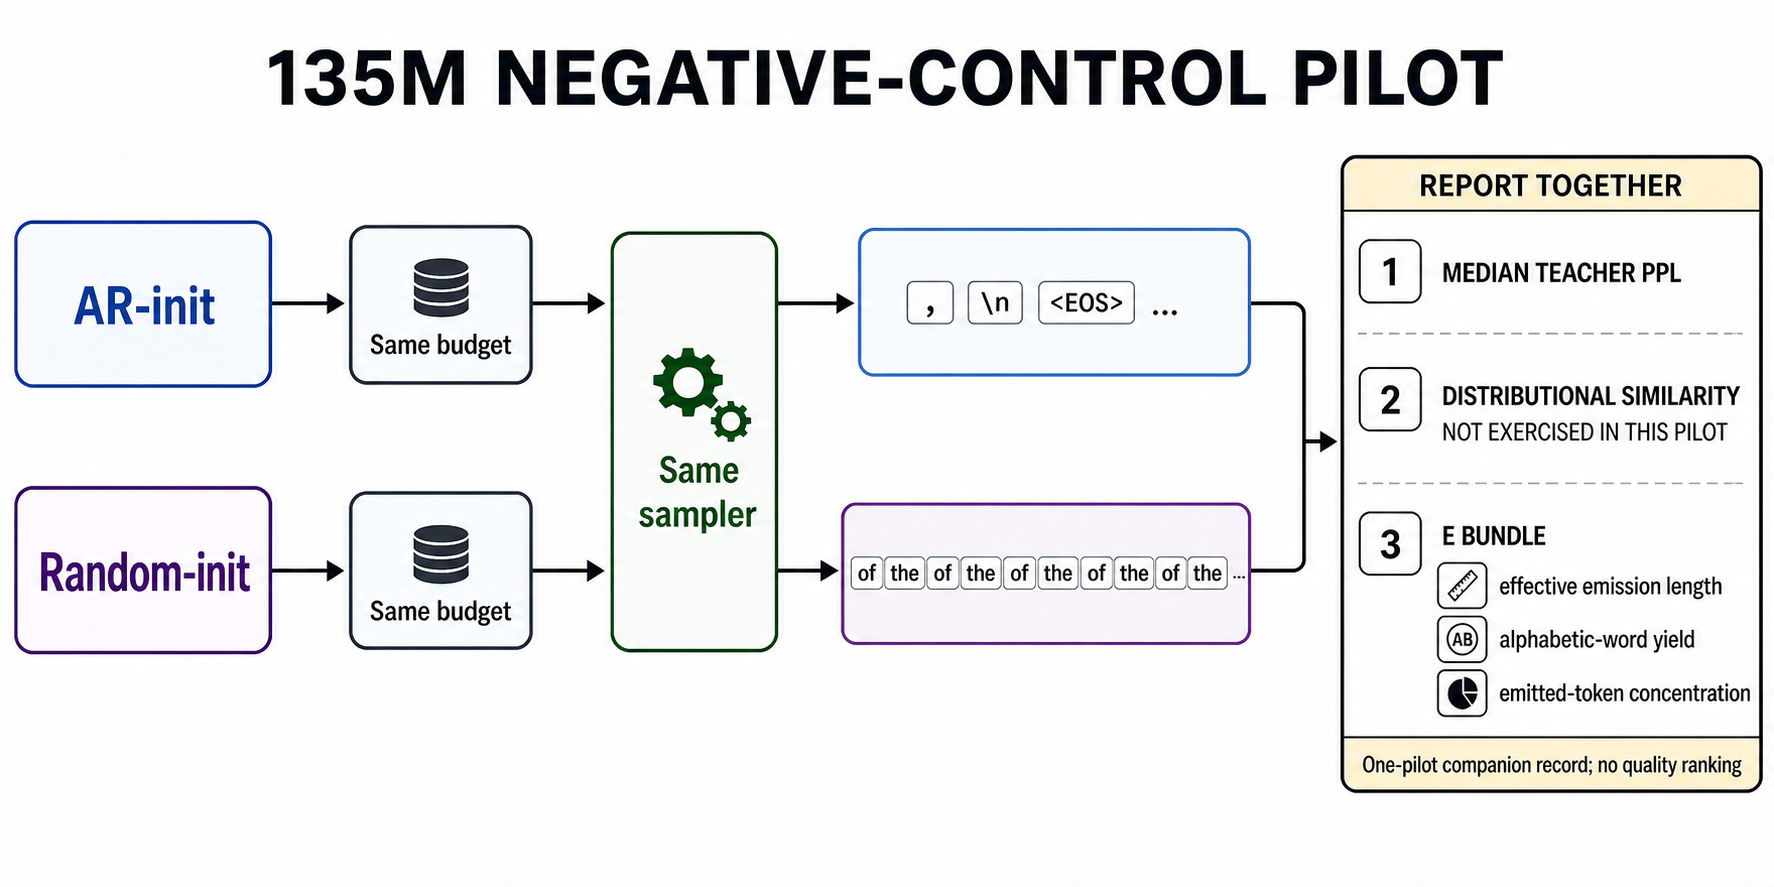
\includegraphics[width=0.96\textwidth]{figures/teaser_reporting_imagegen_r471_v1.png}
  \caption{\textbf{Companion record for this single 135M pilot — the slots of Eq.~\eqref{eq:bundle}.}
  Both arms are degenerate: AR-init stops after punctuation/newline remnants,
  whereas random-init continues as a repeated word stream.  The panel matches
  Eq.~\eqref{eq:bundle} exactly: (i) median teacher PPL; (ii) distributional
  similarity, \emph{not exercised} here because the attempted MAUVE measurement
  is not recorded under this configuration (Section~\ref{sec:ppltrap}); and
  (iii) $\mathcal{E}$, comprising effective emission length, alphabetic-word
  yield, and emitted-token concentration.  No ratio or quality inference is
  made on slot (ii).  Argmax concentration is intentionally excluded because
  the final argmax and emitted distribution decouple in our data
  (Section~\ref{sec:ppltrap}).  This descriptive audit accompanies existing
  measurements; it is neither a new scalar metric nor a quantitative result,
  and all measured values remain in the tables.}
  \label{fig:teaser}
\end{figure*}

\section{Related Work and Evaluation Framing}
\label{sec:related}

\paragraph{Masked diffusion language modeling.}
Masked diffusion objectives can be written as mixtures of masked-language
modeling losses and paired with iterative unmasking samplers
\citep{sahoo2024mdlm}.  LLaDA demonstrated that the paradigm scales to an 8B
parameter model trained from scratch \citep{nie2025llada}; more recent systems
span reusable training frameworks \citep{zhou2026dllm}, continuous embedded
flows \citep{hu2026elf}, and adaptive generation length
\citep{li2025daedal}.  AR-to-diffusion adaptation has already been studied
systematically in the DiffuLLaMA family \citep{gong2025adaptation}; PreDiff-LM
studies pretrained masked diffusion with hybrid attention
\citep{yao2026prediff}, and UNIFUSION studies AR adaptation under a unified
reverse-rate objective \citep{jiang2026unifusion}.  Accordingly, our matched
initialization arms are a small reproducible case study, not a new adaptation
method or training discovery.

\paragraph{Metrics score different projections of emitted text.}
Generated-text PPL scores teacher likelihood; Wang et al.\ show that length,
repetition, and punctuation can distort that score \citep{wang2022ppl}.
MAUVE instead compares generated and human distributions
\citep{pillutla2021mauve}; surface form also matters.  Final-argmax share
describes concentration of the generator's decisions.  Within the 11-source
local verification ledger used for this paper, we did not establish that these
sources report whether the emitted object is a short EOS stub or a long lexical
loop.  Our fields expose those factors on one dLLM bed.  A within-arm,
within-prompt before/after
check (Section~\ref{par:discrim}) establishes complementarity with teacher PPL
only for that pair; discriminative evidence across initializations and prompts
remains unresolved.  Here PPL ranks the arms opposite to the matched four-seed
loss benchmark, but the pre-registered multi-init control reproduces only the
loss-side sign while its degeneration mode varies by draw
(Section~\ref{sec:limitations}).  The conflict therefore motivates the audit
without establishing a quality anchor, discriminative power, or a new metric.
Table~\ref{tab:literature} positions this pilot against the closest locally
verified work.

\begin{table*}[!t]
  \caption{\textbf{Scope comparison with the closest locally verified work.}
  NR means that a field was not measured in this implementation or was not
  established by the frozen local verification ledger; no value is inferred
  from memory.  Relative to \citet{wang2022ppl}, this pilot audits the same
  confounding factors on a matched-initialization dLLM bed and adds the
  within-arm check in Table~\ref{tab:discrim}; no novelty claim rests on an NR cell.}
  \label{tab:literature}
  \centering
  \footnotesize
  \setlength{\tabcolsep}{2.5pt}
  \begin{tabular}{@{}L{0.13\textwidth}L{0.13\textwidth}L{0.14\textwidth}L{0.09\textwidth}L{0.19\textwidth}L{0.10\textwidth}L{0.14\textwidth}@{}}
    \toprule
    Work & Model scale & Training budget & Prompts & Reported evaluation & Human anchor & Emission reporting \\
    \midrule
    Wang et al.\ (2022) & PLM-PPL study & Not a generator-training comparison & NR & PPL; analyzes length, repetition, punctuation & NR & NR \\
    Gong et al.\ (2025) & DiffuLLaMA\newline 7B family & NR & NR & AR-to-diffusion adaptation study & NR & NR \\
    Yao et al.\ (2026) & PreDiff-LM; NR & NR & NR & Pretrained masked diffusion with hybrid attention & NR & NR \\
    Jiang et al.\ (2026) & UNIFUSION\newline NR & NR & NR & Unified reverse-rate AR adaptation & NR & NR \\
    This pilot & 135M & 30.0M tokens/arm; 458 steps & 1 & Two-teacher PPL, MAUVE, argmax and trajectory probes & None & Length, alphabetic yield, top-word share \\
    \bottomrule
  \end{tabular}
\end{table*}

\section{Experimental Protocol}
\label{sec:method}

\subsection{Setup and configuration}
\label{sec:setup}

We fix the training, initialization, generation, scoring, and signal-dump
knobs in Table~\ref{tab:design}; Table~\ref{tab:e1multinit} separately records
the pre-registered multi-initialization control.  This moves reconstructive
values out of prose while preserving their scope and provenance.

\begin{table*}[!t]
  \caption{\textbf{Controlled training and evaluation design.}  Only the
  initialization checkpoint differs between the two principal arms.  The PPL
  teachers and MAUVE configuration are evaluation choices, not independent
  quality anchors.}
  \label{tab:design}
  \centering
  \footnotesize
  \setlength{\tabcolsep}{3pt}
  \renewcommand{\arraystretch}{0.94}
  \begin{tabularx}{\textwidth}{@{}L{0.105\textwidth}Y L{0.105\textwidth}Y@{}}
    \toprule
    Training field & Frozen setting & Evaluation field & Frozen setting \\
    \midrule
    Model / vocab & SmolLM2-135M converted to masked denoising; 49{,}152 base
      tokens plus \texttt{<|mask|>} (49{,}153 total); tied embeddings &
    Checkpoint / prompt & seed-42 checkpoint pair; one prompt, ``To be or not to be.'' \\
    \armB{} draw & Linear/embedding weights i.i.d.\
      $\mathcal{N}(0,(1/24)^2)$; LayerNorm gains 1, biases 0; host ambient RNG
      (no seed argument), hence one fixed draw; raw-HF A2D conversion uses
      \texttt{--random-init} (state dict skipped) before appending the mask row &
    Generation grid & $\tau\in\{0.7,1.0\}$; 32 continuations per arm--temperature
      cell; 128 tokens; 128 denoising steps; block size 32; low-confidence remasking
      as recorded by the hashed sampler entry in the anonymous artifact \\
    Init audit & Per-layer standard deviations within 0.1\% of $1/24$;
      embedding normaltest $p=0.92$, skew $-0.004$, excess kurtosis $0.01$
      ($n=20{,}000$); all 272 tensors differ; no step-0 scalar was logged, so
      the earliest step-10 losses, 9.6009 (A) and 11.2053 (B), are compared
      with $\ln(49{,}153)\simeq10.802$ &
    Length / PPL & Natural length plus caps $L\in\{16,32,48\}$ using
      $\min(n_{\mathrm{full}},L)$; prompt excluded; median PPL under GPT-2
      (124M) and SmolLM2-135M \\
    Data / budget & FineWeb-Edu sample/10BT shards 000/001/003/004;
      $16\!\times\!8\!\times\!458\!\times\!512=30{,}015{,}488$ tokens/arm;
      last logged value at step 450 of 458 &
    MAUVE & \texttt{mauve-text==0.4.0}; GPT-2-large features; holdout shard 005;
      $p=100$, $q=32$, \texttt{num\_buckets=auto}$\rightarrow3$ buckets;
      \emph{not recorded}
      in this pilot; two \armB{} cells identical at
      \texttt{frontier\_integral=1.0} \\
    Optimizer / hardware & AdamW; $10^{-4}$ peak LR; cosine; 10\% warmup;
      bfloat16, ZeRO-2, $8\times$ NVIDIA H20-class accelerators; reference pair 421 s / 0.94 GPU-h;
      three paired repeats 2.40 GPU-h &
    Emission / signal & Median emitted and alphabetic-word counts; corpus
      top-word share; schema v3.1 mask, entropy, max-probability, top-$k$,
      commit, final-argmax, and drift records \\
    MDLM recipe & Uniform $t\in[10^{-3},1)$; linear $\alpha$;
      scheduler-weighted masked CE; \texttt{loss\_norm\_type=token};
      \texttt{right\_shift\_logits=False}; implementation hashes in
      \path{paper/anonymous_artifact/data/reproducibility_anchors.json} &
    Argmax diagnostic & Most frequent final-step strict top-1 over
      $32\times128=4{,}096$ records; distinct from sampled-token frequency \\
    Repeats / seed scope & Paired seeds 42, 2024, 2025, 2026 vary data order
      and training stochasticity on fixed initial weights; arm names were used
      during execution (label-coded, not human double-blind) &
    Provenance & Hashed driver, sampler, serialized training arguments, and
      exact regeneration pointers in
      \path{paper/anonymous_artifact/data/reproducibility_anchors.json} and Appendix~\ref{app:evidence} \\
    \bottomrule
  \end{tabularx}
\end{table*}

\subsection{Matched arms and training budget}
\label{sec:arms}

Both arms use the converted SmolLM2-135M architecture
\citep{allal2025smollm2,zhou2026dllm}.  The \armA{} arm retains pretrained
weights; \armB{} is the fixed, audited from-scratch draw in
Table~\ref{tab:design}.  Crucially, the four paired repeats vary data order and
training stochasticity, not this weight draw, so their loss variance cannot be
transferred to independently drawn random initializations.  To test that gap
we ran a pre-registered multi-init
negative control (Table~\ref{tab:e1multinit}) on three independently drawn
random-initialization checkpoints, each trained under the same 30M-token /
seed-42 data ordering as the two principal arms
(Section~\ref{sec:discussion}).  On the loss side the negative control
reproduces: the paired last-logged-loss gap $(\armB{}_R-\armA{})$ is positive
on all three draws (bootstrap 95\% CI lower bound $>0$), so the
sign-consistency of the principal result does not collapse across random
initializations.  The emission-side degeneration mode, however, is
initialization-dependent: two draws degrade into a repeated-word lexical loop
while the third is a shorter ``gray'' profile, so the emission narrative does
not transfer across draws and is scoped to this effect
(Section~\ref{sec:discussion}; evidence hash and verified fields are in
\path{paper/anonymous_artifact/data/reproducibility_anchors.json}).

\begin{table}[!t]
  \caption{\textbf{Multi-random-init negative control} (pre-registered).
  Fresh seeds 11, 22, and 33 use the principal arms' 30M-token
  seed-42 data ordering.  Loss gaps reproduce on all draws, whereas emission
  mode is initialization-dependent (two loops and one shorter ``gray'' profile).}
  \label{tab:e1multinit}
  \centering
  \footnotesize
  \setlength{\tabcolsep}{2.5pt}
  \begin{tabular}{@{}lccc@{}}
    \toprule
    Draw & Gap $B_R-A$ (nat) & Emission & Words ($\tau{=}0.7$) \\
    \midrule
    \texttt{init-seed}=11 & 2.300 & lexical loop & 125.0 \\
    \texttt{init-seed}=22 & 2.281 & lexical loop & 122.5 \\
    \texttt{init-seed}=33 & 2.272 & gray & 35.0 \\
    \midrule
    bootstrap 95\% CI lower bound & 2.272 ($>0$) & --- & --- \\
    \bottomrule
  \end{tabular}
\end{table}

All token accounting, runtime, logging, objective, scheduler, hardware, and
provenance fields are frozen in Table~\ref{tab:design}; in particular,
``final'' means the step-450 log inside the 458-step run, not a separate
step-458 evaluation.

\subsection{Generation and metric protocol}

Table~\ref{tab:design} gives the complete generation grid.  It is a
single-checkpoint, single-prompt, 32-sample-per-cell pilot rather than a
multi-seed quality estimate.  As preregistered, we report median causal PPL
under GPT-2 and SmolLM2; the median prevents two catastrophic \armA{}
outliers at $\tau=0.7$ from dominating.  SmolLM2 is weight-related to \armA{}
and may share FineWeb-Edu source-domain bias with this experiment, so agreement
with GPT-2 mitigates but does not remove teacher dependence.

Each PPL cell is accompanied by emitted length, alphabetic-word count, and a
pooled corpus top-word share.  The share is an illustrative cell aggregate;
the artifact does not contain a per-continuation concentration distribution,
so we make no continuation-level concentration claim.  These fields describe
the scored emission rather than its quality.  The attempted MAUVE value and
the final-step argmax diagnostic are retained under the same rule: both remain
routine raw records, but neither is used for a pilot quality or capability
inference.  MAUVE is \emph{not recorded} under Table~\ref{tab:design}, and
strict top-1 remains separate from sampled-token frequency at nonzero temperature.

\subsection{Frozen signal layer and probes}
\label{sec:signals}

Schema v3.1 records mask state, entropy, maximum probability, top-$k$
identities and probabilities, commit step, final argmax, and masked-position
drift with explicit dtypes and shapes; evaluation labels remain outside the
trajectory layer.  One dump therefore supports unigram concentration,
tie-aware unresolved-position drift, and committed-position sweep-tail
analyses without another model run.

A fourth analysis applies one instrument to both 135M arms: among currently
masked positions, entropy is scored against whether the current argmax differs
from the eventual final token.  Table~\ref{tab:crossbed} reports the raw AUROC,
trajectory-bootstrap interval ($B=2{,}000$, seed 0), trajectory and step counts,
row support, and permutation calibration (Monte Carlo $B=400$, seed 0).
The calibration estimand is $\mathrm{real}/\mathrm{null95}$, where
$\mathrm{null95}$ is the 95th percentile of the permutation null; a value above
one supplies at most a weak orientation check, not a quality label.

\section{Results}
\label{sec:results}

\subsection{AR initialization preserves a large short-horizon loss advantage}

Figure~\ref{fig:loss} shows the learning curves, and
Table~\ref{tab:seedendpoints} gives every paired endpoint.  The gap
$L_{\text{random}}-L_{\text{AR}}$ is positive for all four data-order seeds,
with mean 2.262 nats and paired-$t$ 95\% CI [2.220, 2.305] ($n=4$).
The nominal one-sided sign test attains only its minimum $p=0.0625$ at $n=4$.
These statistics vary data order and training randomness conditional on fixed
initialization checkpoints, not independent weight draws.

\begin{figure*}[!t]
  \centering
  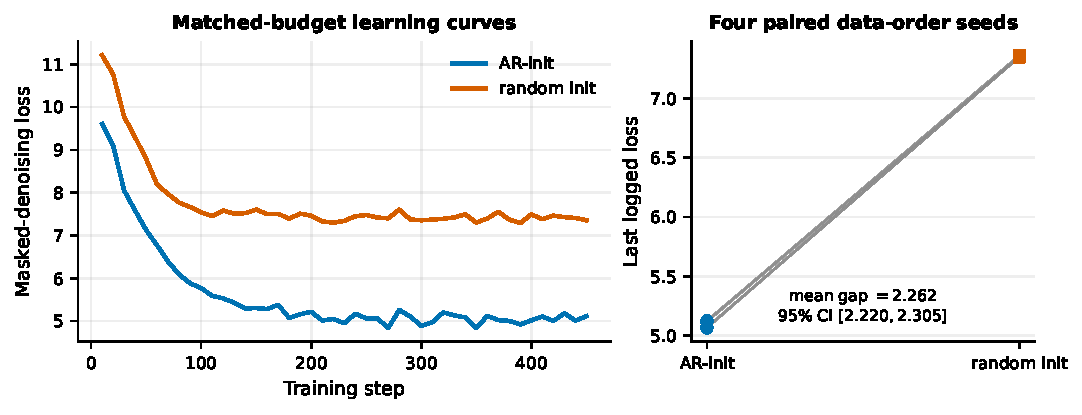
\includegraphics[width=0.96\textwidth]{figures/fig1_loss_curve.pdf}
  \caption{\textbf{Matched-budget training.} Left: both arms receive the same
  458-step, 30.0M-token budget.  Right: last-logged losses and paired-difference
  CI over four data-order seeds; connectors reveal overlapping points.}
  \label{fig:loss}
\end{figure*}

\begin{table}[!t]
  \caption{\textbf{Paired last-logged loss endpoints.}  All four differences
  have the same sign; mean $B-A=2.2623$ nats, paired-$t$ 95\% CI
  [2.2196, 2.3050], and nominal one-sided sign-test $p=0.0625$.}
  \label{tab:seedendpoints}
  \centering
  \footnotesize
  \setlength{\tabcolsep}{4pt}
  \begin{tabular}{@{}rccc@{}}
    \toprule
    Data-order seed & \armA{} & \armB{} & $B-A$ \\
    \midrule
    2024 & 5.0687 & 7.3501 & 2.2814 \\
    2025 & 5.0629 & 7.3522 & 2.2893 \\
    2026 & 5.1243 & 7.3637 & 2.2394 \\
    42   & 5.1159 & 7.3550 & 2.2391 \\
    \bottomrule
  \end{tabular}
\end{table}

Thus, under this recipe, autoregressive weights retain a roughly 2.26-nat
short-horizon advantage after 30M tokens.  Changing curves and one principal
checkpoint per arm preclude convergence-time or asymptotic claims.

\subsection{The degenerate arms differ on emission coordinates}
\label{sec:ppltrap}

Table~\ref{tab:trap} reports the object scored by every perplexity cell.  With
no independent quality anchor, the natural-output medians do not identify a
preferred arm.  The accompanying fields establish only that the two degenerate
arms differ on coordinates outside this pilot's PPL entry; its attempted
MAUVE entry is not recorded.  At $\tau=0.7$, \armA{} is predominantly a short punctuation/newline remnant,
whereas \armB{} continues in a single-word lexical loop; the complete counts
and shares appear in Table~\ref{tab:trap}.

\begin{table*}[!t]
  \caption{\textbf{Perplexity with required emission reporting.} PPL is
  the prompt-excluded median over 32 continuations.  Length and content are
  median word counts; top-word share is pooled over the complete cell and is
  illustrative because no per-continuation distribution was retained.
  Short-stub counts report no-alphabetic-word and at-most-ten-word samples where
  audited.  These coordinates describe the scored object, not a preferred arm.}
  \label{tab:trap}
  \centering
  \footnotesize
  \setlength{\tabcolsep}{3.5pt}
  \begin{tabular}{@{}lccccccc@{}}
    \toprule
    Arm & $\tau$ & \shortstack{SmolLM2\\PPL} & \shortstack{GPT-2\\PPL} &
      \shortstack{Emitted\\length} & \shortstack{Content\\words} &
      \shortstack{Top word\\share} & \shortstack{Short-stub\\counts} \\
    \midrule
    \armA{} & 0.7 & 10.09 & 9.08 & 5.0 & 1.0 & \texttt{and} / 38.0\% &
      \shortstack{9 no-alpha\\25 $\leq10$} \\
    \armB{} & 0.7 & 3.50 & 5.47 & 126.0 & 126.0 & \texttt{of} / 56.8\% & --- \\
    \armA{} & 1.0 & 18.96 & 25.91 & 8.5 & 3.5 & \texttt{and} / 17.5\% & --- \\
    \armB{} & 1.0 & 15.08 & 20.44 & 117.0 & 115.5 & \texttt{of} / 46.9\% & --- \\
    \bottomrule
  \end{tabular}
\end{table*}

\paragraph{A within-arm discrimination check.}
\label{par:discrim}
Table~\ref{tab:discrim} compares \armB{} before and after 458 steps under the
same prompt, seed, $\tau=0.7$, and $32\times128$ protocol.  Teacher PPL moves
by nearly five orders of magnitude, while the untrained draw is a scattered
high-entropy stream and the trained checkpoint a single-token loop.  The PPL
entry alone does not encode the loop, while the emission fields do not encode
teacher fluency.  This
one-arm, one-prompt, one-checkpoint-pair check establishes complementary,
non-redundant information only on that pair, not cross-initialization,
cross-prompt, or cross-checkpoint discrimination power.

\begin{table}[!t]
  \caption{\textbf{Within-arm before/after discrimination check.}  Same
  prompt, seed, $\tau$, and protocol; only training state differs.  PPL is the
  SmolLM2 median and concentration fields use the complete emitted cell.}
  \label{tab:discrim}
  \centering
  \small
  \setlength{\tabcolsep}{3.5pt}
  \begin{tabular}{@{}lcc@{}}
    \toprule
    Coordinate & Untrained (0-step) & Trained (458-step) \\
    \midrule
    SmolLM2 median PPL & 237{,}873.60 & 3.50 \\
    Median emitted words & 82 & 126 \\
    Alphabetic-word yield & 0.991 & 1.000 \\
    Top word / share & \texttt{crossings} / 0.42\% & \texttt{of} / 56.79\% \\
    Top-five cumulative share & 1.25\% & 98.16\% \\
    Distinct-token ratio & 0.941 & 0.023 \\
    \bottomrule
  \end{tabular}
\end{table}

For a common-length view, Table~\ref{tab:lenmatch} caps each sample at
$\min(n_{\mathrm{full}},L)$ while retaining shorter samples at natural length.
The gap survives each SmolLM2 cap, nearly collapses for GPT-2 at $L=32$, and
can reverse at $\tau=1.0$.  Only one of 32 \armA{}, $\tau=0.7$ samples reaches
128 SmolLM2 tokens; its teacher-dependent score is not an estimate.  Hence the
ordering is not robust to teacher, cap, or temperature and supports no robust
quality ranking.

\begin{table*}[!t]
  \caption{\textbf{Length-capped median PPL at $\tau\in\{0.7,1.0\}$.} \armA{}
  and \armB{} use $\min(n_{\mathrm{full}},L)$ teacher tokens; ``full'' is the
  natural $\tau=0.7$ median.  Gap is \armA{} minus \armB{}.}
  \label{tab:lenmatch}
  \centering
  \footnotesize
  \setlength{\tabcolsep}{3.5pt}
  \begin{tabular}{@{}ccccc@{\qquad}ccccc@{}}
    \toprule
    \multicolumn{5}{c}{SmolLM2-135M teacher} &
    \multicolumn{5}{c}{GPT-2 teacher} \\
    $\tau$ & Cap & \armA{} & \armB{} & Gap & $\tau$ & Cap & \armA{} & \armB{} & Gap \\
    \midrule
    0.7 & full & 10.09 & 3.50 & +6.59 & 0.7 & full & 9.08 & 5.47 & +3.61 \\
    0.7 & 16 & 16.31 & 9.54 & +6.77 & 0.7 & 16 & 39.54 & 14.52 & +25.0 \\
    0.7 & 32 & 9.93 & 5.29 & +4.64 & 0.7 & 32 & 9.39 & 8.69 & +0.70 \\
    0.7 & 48 & 10.09 & 4.31 & +5.78 & 0.7 & 48 & 9.08 & 5.92 & +3.16 \\
    1.0 & 16 & 58.19 & 54.67 & +3.52 & 1.0 & 16 & 104.83 & 71.00 & +33.8 \\
    1.0 & 32 & 19.72 & 35.56 & $-15.8$ & 1.0 & 32 & 44.50 & 47.09 & $-2.59$ \\
    1.0 & 48 & 23.54 & 23.21 & +0.33 & 1.0 & 48 & 37.47 & 33.28 & +4.19 \\
    \bottomrule
  \end{tabular}
\end{table*}

The frozen MAUVE configuration is listed in Table~\ref{tab:design}.  Its two
\armB{} cells are numerically identical at the raw frontier integral, so MAUVE
is \emph{not recorded}: no ratio, quality ordering, or capability claim is
formed, while the raw values remain in the artifact for reproduction.

The concentration measurements describe the emitted object rather than an
inferred quality label (Table~\ref{tab:argmax}).  In \armB{}, the strict
final-step top-1 is nearly a single token, while per-position predictive
entropy remains high throughout --- so a ``de-facto argmax filter'' reading
of the committed stream is not supported by the data: the committed token can
disagree with the strict final-step top-1, and argmax concentration and the
emitted distribution decouple.

\begin{table}[!t]
  \caption{\textbf{Argmax concentration and commitment coordinates.}
  Final-step strict top-1 covers 4{,}096 positions ($\tau=0.7$, seed 42,
  128 steps); agreement is zero-tolerance integer-id equality between the
  committed token and strict final-step top-1.}
  \label{tab:argmax}
  \centering
  \small
  \setlength{\tabcolsep}{4pt}
  \begin{tabular}{@{}lcc@{}}
    \toprule
    Coordinate & \armA{} & \armB{} \\
    \midrule
    Records with top-1 = token 260 (\texttt{the}) & --- & 4{,}094 / 4{,}096 \\
    Final-step top-1 entropy (bits) & 3.00 & 0.006 \\
    Final-step top-1 ties & present & zero \\
    Top word in $\tau=0.7$ emission & \texttt{and} / 38.0\% & \texttt{of} / 56.8\% \\
    Per-position predictive entropy (nats) & sweep tail (Fig.~\ref{fig:sweeptail}) & $\approx$7.2--8.1 (flat) \\
    Committed-vs-top-1 agreement & 0.467 & 0.394 \\
    \bottomrule
  \end{tabular}
\end{table}

\subsection{Trajectory records under a failed drift recomputation gate}

The probes give three complementary views.  First, \armB{} has the more
concentrated final-step argmax (Table~\ref{tab:argmax}).  Second, the original
claim that low-confidence layers cause drift is unsupported: the failed
scalar/top-$k$ gate leaves no quantitative error bound for drift localization.
The passing tie-bound and decoding-alignment checks establish only that the
serialization is internally bounded and aligned; they do not recover the
failed counts or a directional mechanism.  Third,
\armA{} falls from high entropy to a mid-trajectory minimum and rises to a
high-entropy residue, whereas \armB{} stays nearly flat
(Figure~\ref{fig:sweeptail}).  This stored-entropy contrast does not use the
failed drift field, but the nearly untrained control (458 steps, final loss
7.36) still cannot distinguish learned structure from the masking schedule.

\begin{figure*}[!t]
  \centering
  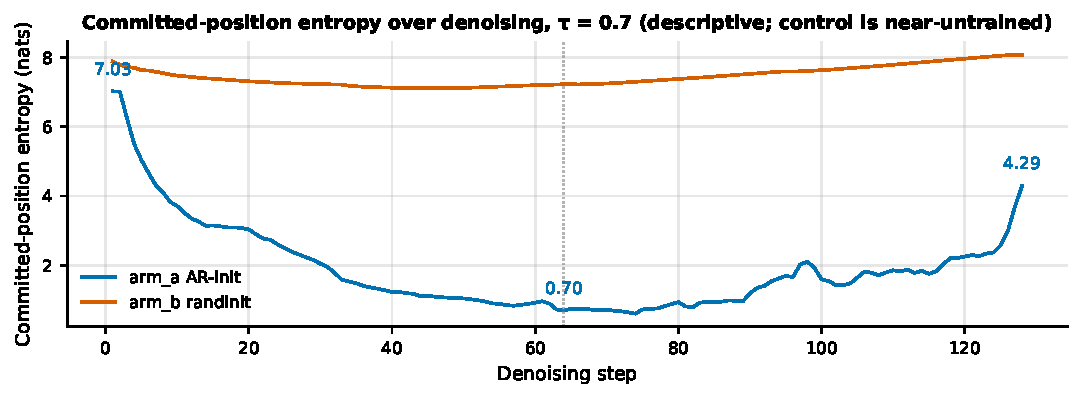
\includegraphics[width=0.96\textwidth]{figures/fig6_sweep_tail.pdf}
  \caption{\textbf{Committed-position entropy over denoising.} The
  AR-init arm develops a mid-trajectory minimum and high-entropy residue;
  random-init remains high.  Curves use frozen v3.1 stored-entropy fields at
  $\tau=0.7$ and do not use the failed scalar/top-$k$ drift recomputation.}
  \label{fig:sweeptail}
\end{figure*}

Table~\ref{tab:driftgate} reports the failed field and the two passing
serialization checks; neither supplies a drift effect or error bound.

\begin{table}[!t]
  \caption{\textbf{Drift recomputation gate.}  Specified top-$k$
  recomputation versus scalar totals at 1\% tolerance.  The failed fields are
  shown only to diagnose the gate; the passing fields support serialization
  alignment, not a drift effect estimate.}
  \label{tab:driftgate}
  \centering
  \small
  \setlength{\tabcolsep}{4pt}
  \begin{tabular}{@{}lcc@{}}
    \toprule
    Quantity & \armA{} & \armB{} \\
    \midrule
    Aggregate scalar/top-$k$ difference & 12.6\% & 18.1\% \\
    Worst single-record relative error & 56.8\% ($57\times$ tolerance) & --- \\
    Tie-bounded consistency gate & pass & pass \\
    Decoding-alignment gate & pass & pass \\
    \bottomrule
  \end{tabular}
\end{table}

\subsection{Masked-entropy orientation check}
\label{sec:crossbed}

The two 135M masked-position entropy results are collected in
Table~\ref{tab:crossbed}.  The previously explored 8B row is omitted because
its checkpoint, prompts, and sampling temperature are not fully specified in
the anonymous artifact.  Off-axis calibration uses a near-one untrained-bed
multiple as a null check.  The raw \armB{} AUROC is 0.45785, with a roughly
0.010-wide interval over a pool of 260{,}064 dependent masked-position rows;
the resampling unit remains only 32 trajectories.  We therefore read it as a
weak, near-null negative orientation, not as strong anti-predictive behavior
or an inverse quality signal.  The \armA{} contrast is 0.68593
[0.6520, 0.7255], also descriptive rather than a quality score.

\begin{table*}[!t]
  \caption{\textbf{Masked-entropy orientation, support, and calibration.}
  Raw AUROC labels whether current argmax differs from the final token; CIs use
  trajectory bootstrap ($B=2{,}000$, seed 0).  Calibration uses 400 seed-0
  permutations and is $\mathrm{real}/\mathrm{null95}$, where $\mathrm{null95}$
  is the permutation-null 95th percentile; it is not an AUROC.  NR denotes a
  field absent from the frozen local artifact.}
  \label{tab:crossbed}
  \centering
  \footnotesize
  \setlength{\tabcolsep}{3.5pt}
  \begin{tabular}{@{}lrrrcc@{}}
    \toprule
    Bed & Traj. & Steps & Masked $n$ & AUROC [95\% CI] & Calib. multiple \\
    \midrule
    \armA{} (135M) & 32 & 128 & 260{,}064 & 0.686 [0.652, 0.725] & 1.334 \\
    \armB{} trained (135M) & 32 & 128 & 260{,}064 & 0.458 [0.453, 0.463] & 1.074 \\
    \armB{} untrained bed & NR & NR & NR & --- & 1.009 \\
    \bottomrule
  \end{tabular}
\end{table*}

\section{Discussion}
\label{sec:discussion}

\paragraph{A negative control is a reporting unit test.}
The random-initialized arm is a unit test for describing distinct degeneration
modes, not a competitive baseline.  For this single 458-step,
single-checkpoint pilot, the within-arm check in Section~\ref{par:discrim}
supports only this companion bundle:
\begin{equation}
  \label{eq:bundle}
  (\text{median teacher PPL},\ \text{distributional similarity},\ \mathcal{E}),
\end{equation}
where $\mathcal{E}$ is effective length, alphabetic yield, and emitted-token
concentration.  The attempted MAUVE value and argmax diagnostic follow the
same retention standard: raw records remain, but neither supports inference.
Slot (ii) is therefore unexercised; argmax is not an emission slot because it
decouples from sampled emissions here (Section~\ref{sec:ppltrap},
Figure~\ref{fig:teaser}).  These fields are not a new metric, and the
multi-init control supports only the loss-side sign, not the PPL/loss ordering.

\paragraph{Loss calibration and generation quality answer different
questions.}
The paired loss gap is statistically repeated; generation uses only seed-42
checkpoints and diagnoses emission coordinates, not production quality.
Neither implies good text, a MAUVE gap, or a quality ranking for \armA{}.

\paragraph{The signal layer is infrastructure, not a new decoder.}
The schema separates masked from committed positions, current argmax from held
token, and top-$k$ ties.  It diagnoses this control; adaptive-decoder accuracy
or efficiency remains outside the evidence.

\section{Limitations}
\label{sec:limitations}

Table~\ref{tab:limits} pairs each frozen boundary with its inferential ceiling.

\begin{table*}[!t]
  \caption{\textbf{Frozen scope and interpretation boundaries.}  Complete
  settings are in Table~\ref{tab:design}; each row states its inferential ceiling.}
  \label{tab:limits}
  \centering
  \footnotesize
  \setlength{\tabcolsep}{4pt}
  \renewcommand{\arraystretch}{0.94}
  \begin{tabularx}{\textwidth}{@{}L{0.13\textwidth}L{0.37\textwidth}Y@{}}
    \toprule
    Axis & Frozen support & Interpretation boundary \\
    \midrule
    Training horizon & 30M tokens/arm; losses still evolving; last log at step
      450 of 458 & No convergence-time speedup or asymptotic ordering. \\
    Paired variation & Four data-order/training seeds with fixed initial
      weights & The paired CI does not estimate random-weight-draw variance. \\
    Multi-init control & Three fresh draws (seeds 11, 22, 33): positive loss
      gap on all three; two lexical loops and one shorter ``gray'' emission &
      Loss-side sign consistency survives this low-power three-draw pilot;
      emission mode is initialization-dependent.  This forward analysis is
      non-gating and not a headline. \\
    Generation & 135M bed; seed-42 checkpoint pair; one prompt;
      $\tau\in\{0.7,1.0\}$; 32 samples/cell; 128-step sampler & No
      extrapolation to other prompts, checkpoints, dLLMs, or LLaDA-8B. \\
    PPL / MAUVE & Length-confounded teacher PPL; one full-length \armA{}
      sample; source-related SmolLM2 teacher; pinned \texttt{mauve-text==0.4.0}
      but automatic three-bucket value not recorded & Ordering is
      teacher-, temperature-, and length-construction-dependent; no MAUVE
      capability or quality conclusion. \\
    Drift / causality & Scalar/top-$k$ totals differ by 12.6--18.1\%; all
      probes observe one sampler & No quantitative error bound, drift effect
      estimate, decomposition, or causal mechanism without a corrected rerun. \\
    Upgrade paths & Only three independent random-weight draws; drift gate
      remains failed & More weight draws and a corrected drift recomputation
      are future evidence upgrades, not results or conditions claimed here. \\
    \bottomrule
  \end{tabularx}
\end{table*}

\paragraph{Ethics and AI assistance.}
No human subjects are involved.  The web corpus retains privacy, licensing,
and representational-bias risks.  AI assisted reorganization and copyediting;
quantitative claims remain artifact-bound and the authors responsible.

\section{Conclusion}

In this 135M negative-control pilot, autoregressive initialization retains a
2.262-nat last-logged loss advantage across four paired data orders, while one
seed-42 generation check contrasts two degenerate emissions.  Effective
length, content yield, and concentration distinguish them; PPL is recorded but
the pinned MAUVE attempt is not.  Without an independent quality anchor, this
is only a companion record for this setting---not a quality ordering, metric
capability, new metric, training discovery, or extrapolation to other dLLMs.

\begingroup
\footnotesize
\section*{Reproducibility Statement}
\label{sec:repro}

The anonymous bundle \path{paper/anonymous_artifact/} has manifest SHA-256
\shachunks{10bde541}{2c17f2e6}{5b0ea123}{0f8a2b2d}{b134c02b}{6eda8b92}{e560211b}{bae6e735}.
It contains emission data, four-seed endpoints, implementation hashes,
regeneration pointers, and the pre-registered multi-init summary (source SHA-256
\shachunks{546af24c}{0267ceba}{08529081}{c0425d9f}{370e0ea0}{d02869dc}{3c98ad49}{0905c1ee}).
No verified external anonymous URL is available at this freeze.
The seed-42 principal safetensors checkpoints have full SHA-256 values
AR-init \shachunks{a618886a}{762eb898}{3cc0821f}{b43261ff}{27f40127}{38e240d0}{0827d0a8}{1d7dd00d}
and random-init
\shachunks{bbfbfb7f}{a4782dea}{8492412e}{dd9bf30e}{edc1940d}{a599848b}{f86d39b8}{c942a509}.
Table~\ref{tab:design} records the random draw's distribution and scale; its
ambient weight seed is missing and differs from training/data-order seed 42.
Step 0 was not logged; the earliest step-10 losses are 9.6009 and 11.2053,
respectively, versus $\ln(49{,}153)\simeq10.802$.

Source commit \texttt{6f21ee9} builds with Tectonic 0.17.0, the pinned ICLR
2026 template, and fixed \texttt{SOURCE\_DATE\_EPOCH}; the rebuild is recorded
in \path{paper/layout/deterministic.json}.  Runtime pins are
\texttt{transformers==4.57.0}, \texttt{datasets==4.2.0},
\texttt{accelerate==1.11.0}, \texttt{sentencepiece==0.2.0}, and
\texttt{mauve-text==0.4.0} on PyTorch/bfloat16, ZeRO-2, and eight anonymized
H20-class accelerators.  The package pin does not make
\texttt{num\_buckets=auto}$\rightarrow3$ byte-reproducible, so the attempted
MAUVE value remains \emph{not recorded}.  Trajectory CIs use $B=2{,}000$,
seed 0; permutation calibration uses $B=400$, seed 0, with
$\mathrm{null95}$ the permutation-null 95th percentile.  All anchors are in
\path{paper/anonymous_artifact/data/reproducibility_anchors.json}.
\endgroup

\bibliographystyle{iclr2026_conference}
% P5_MAIN_TEXT_END
\label{p5:main-text-end}
\begingroup
\small
\setlength{\bibsep}{1pt}
\bibliography{refs}
\endgroup

% Let the short appendix use the space left after the references.
\appendix

\section{Reproducibility and Evidence Index}
\label{app:evidence}

Table~\ref{tab:evidence} maps every headline claim to an on-disk artifact;
the companion \path{paper/anonymous_artifact/README.md} gives field-level JSON
pointers, commands, and scope restrictions.

\begin{table}[!h]
  \caption{\textbf{Claim-to-artifact evidence map.}  Each headline claim is
  bound to a primary on-disk artifact and its regeneration or audit entry;
  \protect\path{paper/anonymous_artifact/README.md} carries the field-level JSON
  pointers.}
  \label{tab:evidence}
  \centering
  \footnotesize
  \setlength{\tabcolsep}{4pt}
  \renewcommand{\arraystretch}{0.94}
\begin{tabular}{@{}L{0.18\textwidth}L{0.38\textwidth}L{0.36\textwidth}@{}}
  \toprule
  Claim & Primary artifact & Regeneration / audit \\
  \midrule
  Training budget, curves, paired gap, and CI &
  \path{paper/anonymous_artifact/}\newline
  \path{data/multiseed_summary.json} &
  \path{scripts/multiseed_postprocess.py};\newline
  \path{data/reproducibility_anchors.json} \\
  PPL, degraded MAUVE, emission coordinates, and length checks &
  \path{paper/anonymous_artifact/data/}\newline
  \path{phase2_summary.json};\newline\path{emission_coords.json} &
  \path{scripts/phase2_emission_coords.py};\newline
  \path{scripts/phase2_gen_ppl_lengthmatched.py} \\
  Argmax, drift, and sweep-tail probes &
  \path{paper/anonymous_artifact/data/}\newline
  \path{unigram.json}; \path{drift_layer.json};\newline
  \path{sweep_tail.json} &
  Frozen v3.1 fields; drift failure retained as a gate diagnostic \\
  Masked-entropy AUROC &
  \path{paper/anonymous_artifact/}\newline\path{results/cross_paradigm.json} &
  \path{data/reproducibility_anchors.json} \\
  \bottomrule
\end{tabular}
\end{table}

\end{document}
